\documentclass[UTF8]{ctexbeamer}	%handout
\usetheme{Madrid}
%\usecolortheme{whale}
\usecolortheme{beaver}
\usefonttheme{professionalfonts}

\usepackage{graphicx}
\graphicspath{{fig/}}
\usepackage{subfigure}

%\usepackage{amsmath,amssymb,amsthm}
\usepackage{mathtools}
\usepackage{siunitx}
\usepackage{witharrows}

\usepackage{xcolor}
\definecolor{fall-green}{HTML}{008000}

\usepackage{tikz}
\usetikzlibrary{decorations.pathreplacing}
\newcommand{\tikzmark}[1]{\tikz[overlay,remember picture] \node[baseline] (#1) {};}
\tikzset{My Node Style/.style={midway, right, xshift=3.0ex, align=left, font=\small, draw=blue!50, thin, fill=cyan!25, text=black}}
\newcommand\VerticalBrace[4][]{%
	% #1 = draw options
	% #2 = top mark
	% #2 = bottom mark
	% #4 = label
	\draw[decorate,decoration={brace, amplitude=1ex}, #1]
	([yshift=1.5ex]#2.east)  -- (#3.east)
	node[My Node Style] {#4};
}
\newcommand\RightArrow[3][]{%
	% #1 = draw options
	% #2 = mark
	% #3 = label
	\draw[<-, shorten >=0.1cm, #1]
	([shift={(0.8cm,0.5ex)}]#2.east)  -- ([shift={(0.0cm,0.5ex)}]#2.east)
	node[My Node Style] {#3};
}

\newenvironment<>{question}[1][]{
	\begin{exampleblock}#2{问题}}{\end{exampleblock}}
\newenvironment<>{answer}[1][]{
	\begin{alertblock}#2{答案}}{\end{alertblock}}

\AtBeginSection[]
{
	\begin{frame}
	\tableofcontents[currentsection]
\end{frame}
}
\AtBeginSubsection[]
{
	\begin{frame}
		\tableofcontents[currentsection,currentsubsection]
	\end{frame}
}

\author{王介哲}
\institute{优才教育}
\title{数的历史与发展}
%\date{\today}
%\logo{\includegraphics[height=1cm]{seal.jpg}}

\begin{document}

\frame{\titlepage}

\frame{\tableofcontents}

\section{数的诞生}

\begin{frame}
	\begin{block}{你能想到那些简单的计数方式?}\pause
		\begin{itemize}[<+-| alert@+>]
			\item 绳子打结
			\item 骨头穿孔
			\item 泥板刻痕
			\item ……
		\end{itemize}
	\end{block}
\end{frame}

\begin{frame}\frametitle{最早的数字}
	\begin{columns}[c]
		\begin{column}{0.6\textwidth}
			\begin{question}
				最早的数字出现在什么时候?\\
				\begin{enumerate}[(A)]
					\item 十万年前
					\item 三万年前
					\item 一万年前
					\item 五千年前
				\end{enumerate}
			\end{question}\pause
			\begin{answer}
				(B)\\
				数的第一次使用可以追溯到大约公元三万年前,迄今为止发现的最早的例子是在南非的一个洞穴里。
			\end{answer}\pause
		\end{column}
	\begin{column}{0.3\textwidth}
		\begin{figure}
			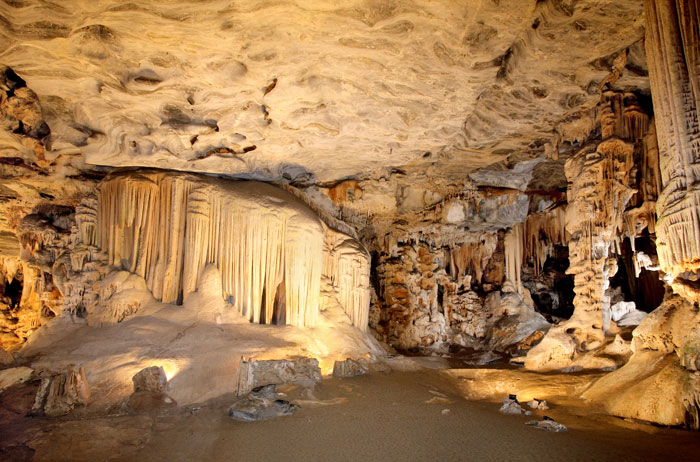
\includegraphics[width=\textwidth]{cango_cave_1.jpg}\\
			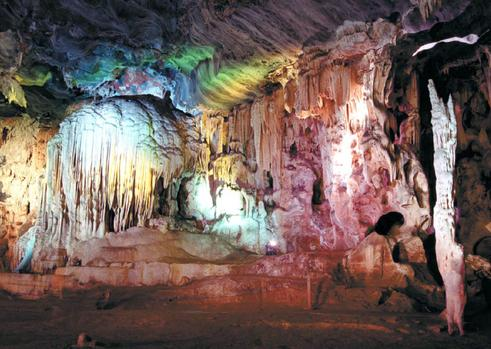
\includegraphics[width=\textwidth]{cango_cave_2.jpg}
			\caption{南非·甘果洞}
		\end{figure}
	\end{column}
	\end{columns}
\end{frame}

\begin{frame}{一则笑话}
	\begin{block}{谁说出的数字大?}\pause
	{
		两个匈牙利贵族决定做一次数数游戏——谁说出的数字最大谁赢。\\
		``好,''一个贵族说,``你先说把!''\\
		另一个绞尽脑汁想了好久,终于说出他所想到的最大数字:``3''。\\
		现在轮到第一个动脑筋了。苦思冥想了更久,他表示弃权说:``你赢啦!''\\
		\rightline{——伽莫夫《从一到无穷大》}
	}
	\end{block}\pause
	\begin{question}
		最大的数是多少?
	\end{question}
\end{frame}
\section{古代计数方法}

\subsection{古埃及}

\begin{frame}\frametitle{古埃及}
	\begin{figure}\centering
		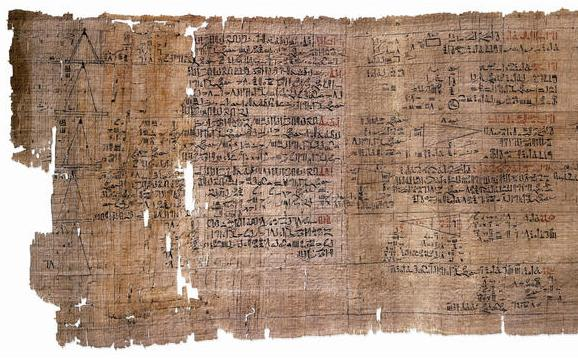
\includegraphics[width=0.8\textwidth]{Rhind_Mathematical_Papyrus.jpg}
		\caption{莱因德数学纸草书,著于约公元前1700年}
	\end{figure}
\end{frame}

\begin{frame}\frametitle{古埃及}
	\begin{block}{莱因德数学纸草书}
		总长525厘米、高33厘米,现藏大英博物馆。\\
		纸草书的内容分两部分:前面是一个分数表,后面是84个数学问题和一段无法理解的话(也称为问题85)。\\
		问题涉及素数、合数和完全数,算术,几何,调和平均数以及简单筛法等概念,其中还有对$\pi$的简单计算,所得值为3.1605。
	\end{block}
\end{frame}

\begin{frame}{古埃及}
	\begin{figure}\centering
		\subfigure{
			\includegraphics<1->[width=0.45\textwidth]{numbers1.jpg}
		}
		\subfigure{
			\includegraphics<2>[width=0.45\textwidth]{numexam21.jpg}
		}
	\caption{古埃及数字}
	\end{figure}
\end{frame}

\begin{frame}{古埃及}
\begin{exampleblock}{这是多少?}
	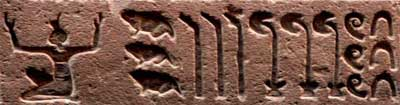
\includegraphics[width=0.8\textwidth]{numbers2.jpg}
\end{exampleblock}\pause
\begin{answer}
	1,333,330
\end{answer}
\end{frame}

\begin{frame}{古埃及}
	\begin{figure}\centering
		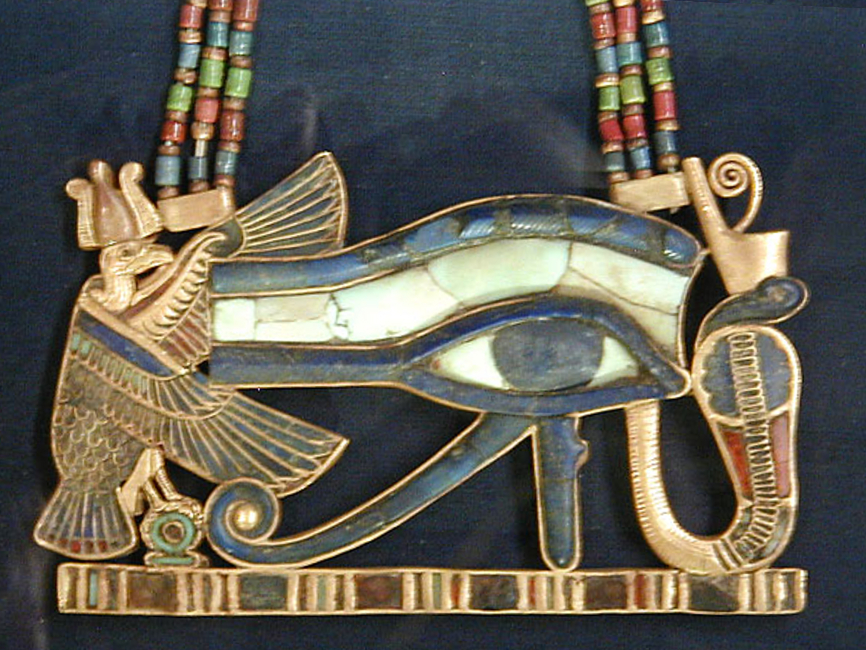
\includegraphics[width=0.45\textwidth]{Wedjat_(Udjat)_Eye_of_Horus_pendant.jpg}
		\caption{荷鲁斯之眼}
	\end{figure}
\end{frame}

\begin{frame}{古埃及}
	\begin{block}{荷鲁斯之眼}
		荷鲁斯之眼顾名思义,它是鹰头神荷鲁斯的眼睛。\\
		荷鲁斯的右眼象征完整无缺的太阳,依据传说,因荷鲁斯战胜赛特,右眼有著远离痛苦,战胜邪恶的力量。\\
		荷鲁斯的左眼象征有缺损的月亮,依据传说,荷鲁斯后来将左眼献给欧西里斯,因而左眼亦有分辨善恶、捍卫健康与幸福的作用,亦使古埃及人也相信荷鲁斯的左眼具有复活死者的力量。
	\end{block}
\end{frame}

\begin{frame}{古埃及}
	\begin{figure}\centering
		\subfigure{
			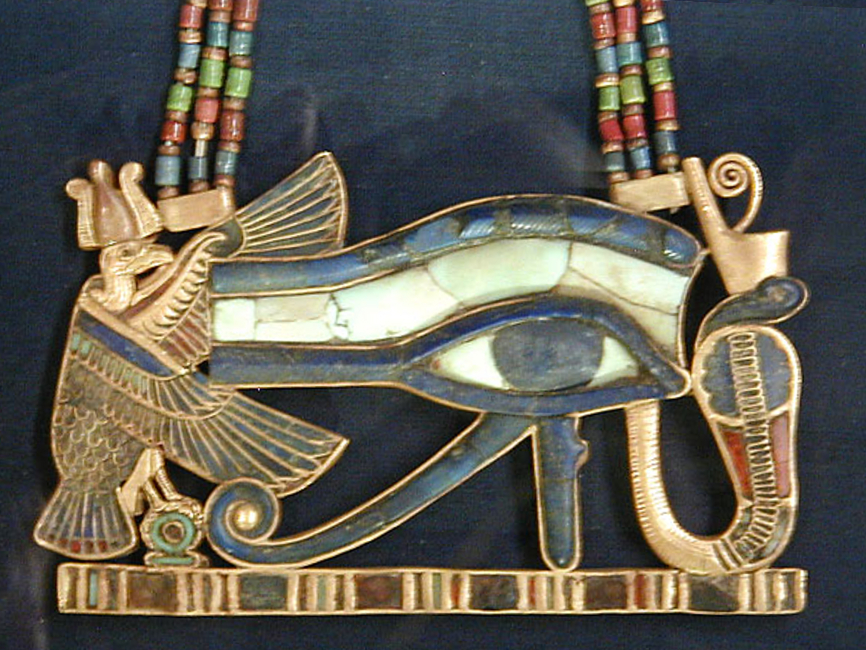
\includegraphics[width=0.45\textwidth]{Wedjat_(Udjat)_Eye_of_Horus_pendant.jpg}
		}
		\subfigure{
			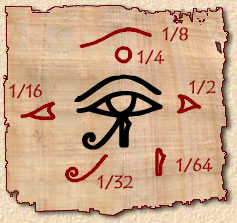
\includegraphics[width=0.47\textheight]{frac.jpg}
		}
		\caption{荷鲁斯之眼}
	\end{figure}
\end{frame}

\subsection{古巴比伦}

\begin{frame}\frametitle{古巴比伦}
	\begin{figure}\centering
		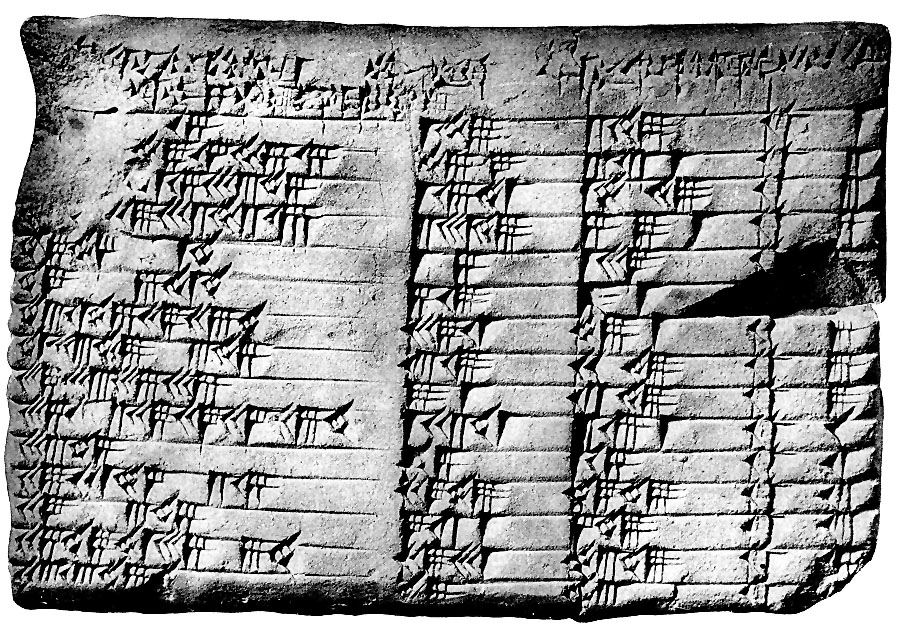
\includegraphics[width=0.8\textwidth]{Plimpton_322.jpg}
		\caption{普林顿322,刻于约公元前1800年}
	\end{figure}
\end{frame}

\begin{frame}\frametitle{古巴比伦}
	\begin{block}{普林顿322}
		普林顿 322为古巴比伦的一个泥板,约13厘米宽,9厘米高,2厘米厚,现藏于哥伦比亚大学。\\
		泥板上有一个四个行十五列和楔形文字组成的表格,表格列出了15组勾股数。
	\end{block}
\end{frame}

\begin{frame}\frametitle{古巴比伦}
	\begin{figure}\centering
		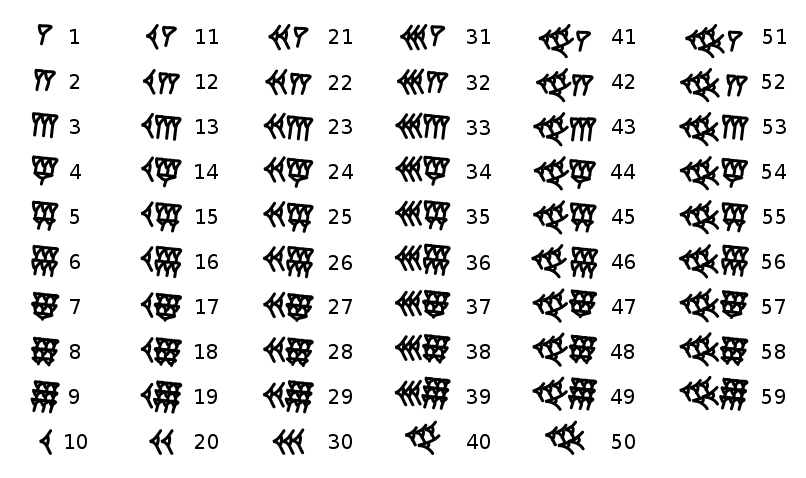
\includegraphics[height=0.5\textheight]{Babylonian_numerals.png}
		\caption{巴比伦数字}
	\end{figure}
\end{frame}

%\begin{frame}\frametitle{古巴比伦}
%	\begin{columns}[c]
%		\begin{column}{.5\textwidth}
%			\begin{figure}\centering
%				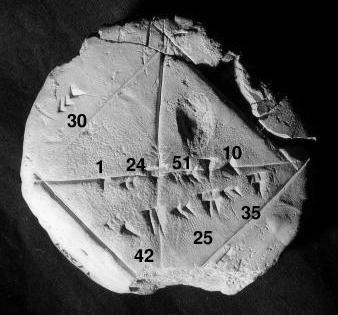
\includegraphics[width=.8\textwidth]{Ybc7289-bw.jpg}
%				\caption{巴比伦泥板 YBC 7289}
%			\end{figure}
%		\end{column}
%		\begin{column}{.5\textwidth}
%			对角线表示2的平方根,用4个六十进制的数字表示:
%			\[1+\dfrac{24}{60}+\dfrac{51}{60^2}+\dfrac{10}{60^3}=1.41421296...\]
%		\end{column}
%	\end{columns} 
%\end{frame}

\subsection{古印度}

\begin{frame}\frametitle{古印度}
	\begin{figure}\centering
		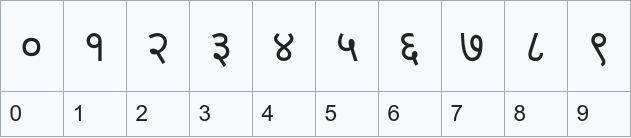
\includegraphics[width=0.8\textwidth]{Selection_110.png}
		\caption{天城文数字}
	\end{figure}
\end{frame}

\subsection{古中国}

\begin{frame}\frametitle{古中国}
	\begin{figure}\centering
		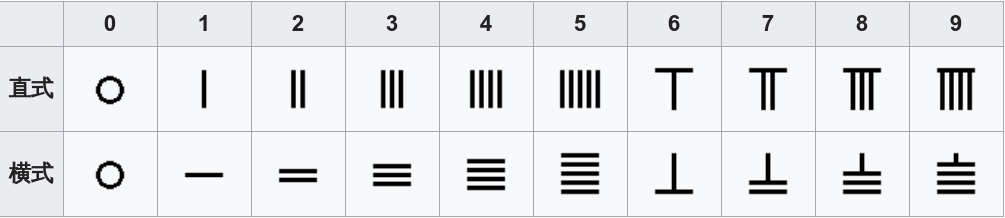
\includegraphics[width=0.5\textwidth]{Selection_111.png}
		\caption{算筹正数}
	\end{figure}\pause
	\begin{figure}\centering
		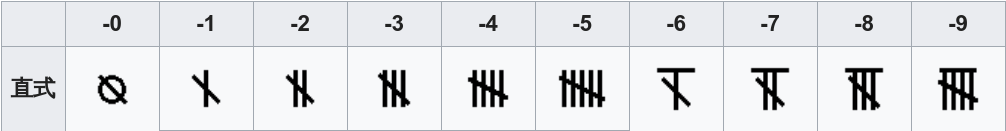
\includegraphics[width=0.5\textwidth]{Selection_112.png}
		\caption{负数}
	\end{figure}\pause
	\begin{figure}\centering
		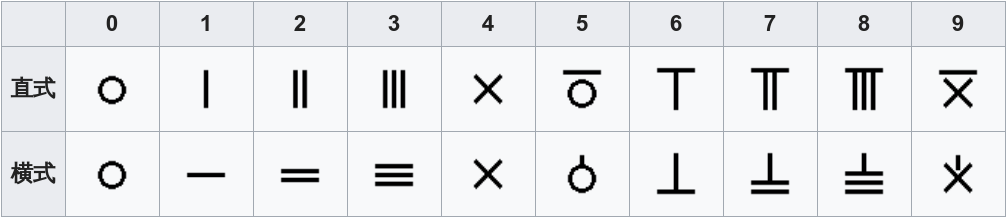
\includegraphics[width=0.5\textwidth]{Selection_113.png}
		\caption{南宋正筹码}
	\end{figure}
\end{frame}

\begin{frame}{古中国}
	\begin{figure}
		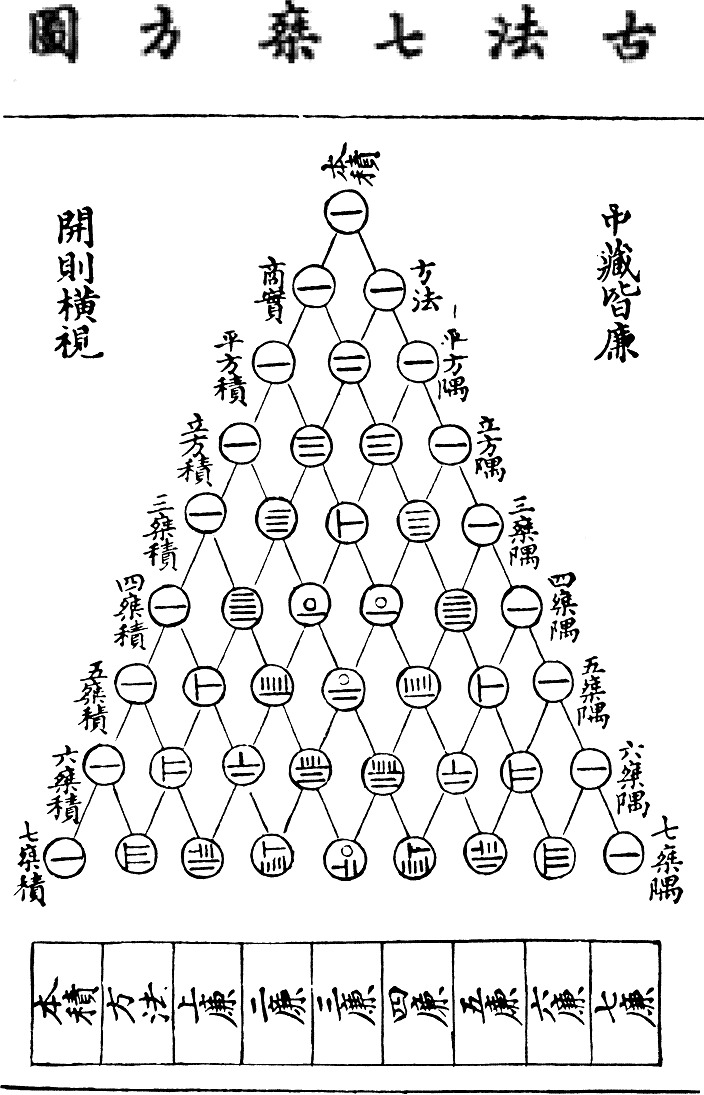
\includegraphics[height=0.7\textheight]{Yanghui_triangle.jpg}
		\caption{杨辉三角}
	\end{figure}
\end{frame}
\section{罗马数字}

\begin{frame}\frametitle{罗马数字}
	罗马数字共有7个:\\
	\vspace{0.5em}
	\renewcommand{\arraystretch}{1.5}
	\begin{tabular}{| *{8}{c|}}
		\hline
		罗马数字 & \alert{I} & \alert{V} & \alert{X} & \alert{L} & \alert{C} & \alert{D} & \alert{M} \\ \hline
		数值 & 1 & 5 & 10 & 50 & 100 & 500 & 1000 \\ \hline
	\end{tabular}\pause
	\begin{block}{拼写规则}
		\begin{itemize}
			\item 右加左减
			\item 加线乘千
			\item 数码限制 
		\end{itemize}
	\end{block}
\end{frame}

\begin{frame}\frametitle{罗马数字}
	\begin{block}{右加左减}\pause
		\begin{itemize}[<+- | alert@+>]
			\item 在较大的罗马数字的右边记上较小的罗马数字,表示大数加小数
			\item 在较大的罗马数字的左边记上较小的罗马数字,表示大数减小数
			\item 左减的数字有限制,仅限于I、X、C\\
				比如45不可以写成VL,只能是XLV
			\item 左减时不可跨越一个位值\\
				比如,99不可以用IC(\texttt{100-1})表示,而是用XCIX( \texttt{[100-10]+[10-1]})表示。
		\end{itemize}
	\end{block}
\end{frame}

\begin{frame}\frametitle{罗马数字}
	\begin{block}{加线乘千}\pause
		\begin{itemize}[<+-| alert@+>]
			\item 在罗马数字的上方加上一条横线,表示将这个数乘以1000,即是原数的1000倍
			\item 同理,如果上方有两条横线,即是原数的1000000( $1000^2$)倍
		\end{itemize}
	\end{block}
\end{frame}

\begin{frame}\frametitle{罗马数字}
	\begin{block}{数码限制}\pause
		\begin{itemize}[<+-| alert@+>]
			\item 同一数码最多只能连续出现三次,如40不可表示为XXXX,而要表示为XL
			\item 例外:由于IV是古罗马神话主神朱庇特(即IVPITER,古罗马字母里没有J和U)的首字,因此有时用IIII代替IV
		\end{itemize}
	\end{block}
\end{frame}

\begin{frame}
	%	\frametitle{罗马数字}
	\begin{block}{右加左减}
		\begin{itemize}
			\item 在较大的罗马数字的右边记上较小的罗马数字,表示大数加小数
			\item 在较大的罗马数字的左边记上较小的罗马数字,表示大数减小数
			\item 左减的数字有限制,仅限于I、X、C
			\item 左减时不可跨越一个位值
		\end{itemize}
	\end{block}
	\begin{exampleblock}{加线乘千}
		\begin{itemize}
			\item 在罗马数字的上方加上一条横线,表示原数的1000倍
			\item 同理,如果上方有两条横线,即是原数的1000000倍
		\end{itemize}
	\end{exampleblock}
	\begin{alertblock}{数码限制}
		\begin{itemize}
			\item 同一数码最多只能连续出现三次
			\item 例外:有时可以用IIII代替IV
		\end{itemize}
	\end{alertblock}
\end{frame}

\begin{frame}\frametitle{罗马数字}
	\begin{columns}[c]
		\begin{column}{.45\textwidth}
			\begin{exampleblock}{罗马数字 -> 数值:}
				\begin{itemize}
					\item<2-> VIII
					\item<4-> XIV
					\item<6-> LX
					\item<8-> XCIX
					\item<10-> CXCIX
					\item<12-> M$\overline{\text{V}}$
				\end{itemize}
			\end{exampleblock}
		\end{column}
		\begin{column}{.45\textwidth}
			\begin{alertblock}{答案:}
				\begin{itemize}
					\item<3-> 8
					\item<5-> 14
					\item<7-> 60
					\item<9-> 99
					\item<11-> 199
					\item<13-> 4000
				\end{itemize}
			\end{alertblock}
		\end{column}
	\end{columns}
\end{frame}

\begin{frame}\frametitle{罗马数字}
\begin{columns}[c]
\begin{column}{.45\textwidth}
	\begin{exampleblock}{数值 -> 罗马数字:}
		\begin{itemize}
			\item<2-> 19
			\item<4-> 145
			\item<6-> 361
			\item<8-> 1437
			\item<10-> 8191
			\item<12-> 65537
		\end{itemize}
	\end{exampleblock}
\end{column}
\begin{column}{.45\textwidth}
	\begin{alertblock}{答案:}
		\begin{itemize}
			\item<3-> XIX
			\item<5-> CXLV
			\item<7-> CCCLXI
			\item<9-> MCDXXXVII
			\item<11-> $\overline{\text{V}}$MMMCXCI
			\item<13-> $\overline{\text{L}}\overline{\text{X}}\overline{\text{V}}$DXXXVII
		\end{itemize}
	\end{alertblock}
\end{column}
\end{columns}
\end{frame}
\section{正数和负数}

\begin{frame}\frametitle{为什么会存在负数?}\pause
	\begin{block}{1、日常生活需要}\pause
		\begin{itemize}
			\item 建国以后北京历史最低温度:零下 \SI{27.4}{\degreeCelsius}(1966) \quad\pause \underline{\SI{-27.4}{\degreeCelsius}}\pause
			\item 中国大陆最低点(新疆吐鲁番艾丁湖洼地)海拔:海平面以下$154.31$米 \quad\pause \underline{$-154.31\text{m}$}\pause
			\item 2018年5月9日上证指数:下跌$2.35$个点,收于3159.15个点\quad\pause \underline{\color{fall-green}$-2.35$}\pause
			\item 支出,负资产……
		\end{itemize}
	\end{block}	
\end{frame}

\begin{frame}\frametitle{为什么会存在负数?}
	\begin{block}{2、数学的对称性}\pause
		正整数具有如下运算规律:
		\begin{enumerate}
			\item 加法交换律:$a + b = b + a$
			\item 加法结合律:$(a + b) + c = a + (b + c)$
			\item 乘法交换律:$a \times b = b \times a$
			\item 乘法分配率:$a \times (b + c) = a \times b + a \times c$
			\item 加法单位元:$a + 0 = 0 + a = 0$
			\item 乘法零元:$a \times 0 = 0 \times a = 0$
		\end{enumerate}
	\end{block}	\pause
	\begin{question}
		什么数满足:$\boxed{?} + 1 = 0$
	\end{question}
\end{frame}

\begin{frame}\frametitle{为什么会存在负数?}
	解方程:
	\[\begin{WithArrows}
		x + 1 &= 0 \\ \pause
		x &= 0 - 1 \pause \Arrow{省去 $0$} \\
		x &= -1
	\end{WithArrows}\] \pause
	\begin{definition}{\alert{负整数}}
		设 $a$ 为整数,则
		\[-a = 0 - a\]
	\end{definition}\pause
	\vspace{1ex}
	对于负分数,我们可以作同样的定义。
\end{frame}

\begin{frame}{负数的运算法则}\pause
	\begin{block}{加减法}\pause
		\begin{enumerate}[<+- | alert@+>]
			\item $a + (-b) = a + (0-b) = (a + 0) - b = a - b$
			\item $-a + b = (-a) + b = b + (-a) = b - a$
			\item $ -a + (-b) = (-a) + (-b) = (-a) - b = 0 - a - b = 0 - (a + b) = -(a + b)$
			\item $a - (-b) = a - (0 - b) = a - 0 + b = a + b$
			\item $-a - (-b) = -a + b = b - a$
		\end{enumerate}
	\end{block}
	\begin{alertblock}<8>{规律}
		\qquad 负号$\approx$减号
	\end{alertblock}
\end{frame}

\begin{frame}{负数的运算法则}
	\begin{center}
		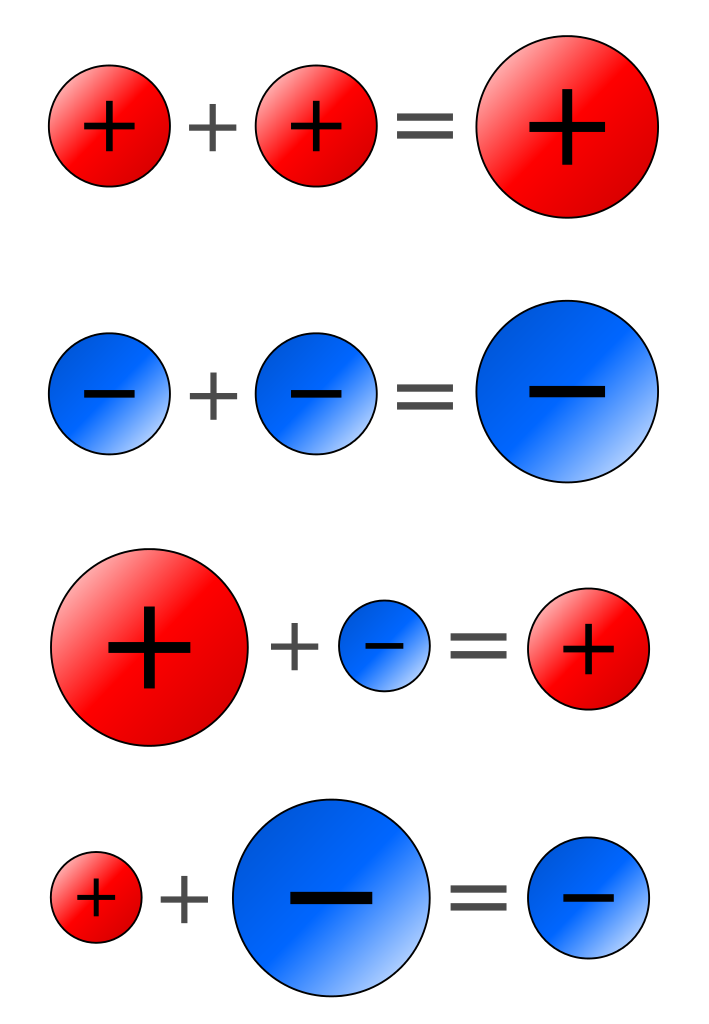
\includegraphics[height=0.8\textheight]{AdditionRules.png}
	\end{center}
\end{frame}

\begin{frame}{负数的运算法则}
	\begin{block}{乘法} \pause
		\begin{enumerate}[<+- | alert@+>]
			\item $a \times (-b) = a \times (0 - b) = a \times 0 - a \times b = 0 - a \times b = - a \times b$
			\item $(-a) \times b = b \times (-a) = - b \times a = - a \times b$
			\item $(-a) \times (-b) = - a \times (-b) = - (- a \times b) = a \times b$
			\item $(-a) \div b = - a \div b$
			\item $a \div (-b) = - a \div b$
			\item $(-a) \div (-b) = a \div b$
		\end{enumerate}
	\end{block}
	\begin{alertblock}<8>{规律}
		\qquad 负负得正,奇负偶正
	\end{alertblock}
\end{frame}

\begin{frame}
	\begin{alertblock}{注意}
		正负是相对的!
	\end{alertblock}
\end{frame}
\section{有理数}

\begin{frame}
	\begin{block}{}
		我们学过那些数?
	\end{block}\pause
	\begin{itemize}
		\item 自然数
		\item 整数
		\item 小数
		\item 分数
		\item $\pi$
	\end{itemize}
\end{frame}

\begin{frame}
	\begin{block}{}
		还记得小数的分类吗?
	\end{block}\pause
	\vspace{1ex}
	\(
	\text{小数}
	\begin{dcases}
	\text{有限小数} \hspace{9em} \tikzmark{Q top} \hspace{6em} \tikzmark{R top} \\
	 \text{无限小数} \pause
	\begin{dcases}
	\text{无限循环小数} \hspace{2em} \tikzmark{Q bottom} \\ 
	\text{无限不循环小数} \tikzmark{NQ} \hspace{7em} \tikzmark{R bottom}
	\end{dcases}
	\end{dcases}
	\)\pause
	\begin{tikzpicture}[overlay,remember picture]
		\VerticalBrace[thick, blue]{Q top}{Q bottom}{有理数}
	\end{tikzpicture} \pause
	\begin{tikzpicture}[overlay,remember picture]
		\RightArrow[thick,blue]{NQ}{无理数}
	\end{tikzpicture} \pause
	\begin{tikzpicture}[overlay,remember picture]
		\VerticalBrace[thick, blue]{R top}{R bottom}{实数}
	\end{tikzpicture}
\end{frame}

\begin{frame}
	\begin{block}{}
		能不能给``有理数''下个定义?
	\end{block}\pause
	注意:有限小数 $\to$ 整数或分数,无限循环小数 $\to$ 分数;\\ \pause
	\vspace{1ex}
	\qquad $\text{整数} = \dfrac{\text{整数}}{1}$,$\text{分数} = \dfrac{\text{整数}}{\text{整数}}$ \pause
	\begin{definition}{\alert{有理数}}
		能表示为整数之比的数。
	\end{definition} \pause
	\[\text{有理数}
		\begin{dcases}
			\text{整数} \uncover<6->{\quad 0, 1, 4, -3, \frac{6}{6}, \frac{40}{8}, 600\%, \cdots} \\
			\text{分数} \uncover<7->{\quad \frac{1}{2}, \frac{4}{6}, -\frac{7}{12}, 3.14, -0.05, \cdots}
		\end{dcases}
	\]
\end{frame}

\begin{frame}
	\begin{block}{}
		如何将有理数分类?
	\end{block} \pause
	\begin{columns}[c]
		\begin{column}{0.5\textwidth}
			\[\text{有理数}
				\begin{dcases}
					\text{整数} \uncover<3->{\begin{dcases} \text{正整数} \\ 0 \\ \text{负整数} \end{dcases}} \\
					\text{分数} \uncover<4->{\begin{dcases} \text{正分数} \\ \text{负分数} \end{dcases}}
				\end{dcases}
			\]
		\end{column} \pause
	\begin{column}{0.5\textwidth}
		\uncover<5->{\[\text{有理数}
			\begin{dcases}
				\text{正有理数} \uncover<6->{\begin{dcases} \text{正整数} \\ \text{正分数} \end{dcases}} \\
				0 \\
				\text{负有理数} \uncover<7->{\begin{dcases} \text{负整数} \\ \text{负分数} \end{dcases}}
			\end{dcases}
		\]}
	\end{column}
	\end{columns}
\end{frame}

\end{document}